\documentclass[a4paper]{article}
\usepackage{fancyhdr}
\usepackage{lastpage}
\usepackage{graphicx}
\usepackage{twocolceurws}
\usepackage{amsmath}
\usepackage{tabularx}
\usepackage{graphicx}
\usepackage{multirow}
\usepackage{rotating}
\usepackage{url}
\usepackage[margin=1in,footskip=0.5in]{geometry}  % Adjust the footskip value as needed

% Configure the fancyhdr package
\pagestyle{fancy}
\fancyhf{}
\fancyfoot[C]{Page \thepage\ of \pageref{LastPage}}


\title{Semantic Segmentation of Urban Drone Imagery}

\institution{University of Milan-Bicocca}

\author{
\textbf{Andrea Palmieri} \\  a.palmieri13@campus.unimib.it \\ Matricula  921785
}

\begin{document}
\maketitle

\begin{abstract}
This paper presents a comparative study of semantic segmentation techniques applied to urban drone imagery using the \textit{Semantic Drone Dataset}. The study focuses on evaluating the performance of three encoder architectures—\textit{EfficientNetB5}, \textit{ResNet34}, and \textit{MobileNetV2}—integrated within the \textit{DeepLabv3+} framework. The primary objective is to assess the feasibility of these models for real-time deployment on drones, particularly for tasks like autonomous navigation and infrastructure monitoring in urban environments. The results indicate that while \textit{EfficientNetB5} delivers the highest segmentation accuracy, \textit{MobileNetV2} offers a compelling balance between performance and computational efficiency, making it well-suited for use on resource-constrained platforms such as drones. 
\end{abstract}

\section{Introduction}
\subsection{Background}
Semantic segmentation is a critical task in the field of computer vision, especially when applied to drone imagery for urban environments. This technique is essential for enabling drones to autonomously navigate complex urban areas, where accurate identification of various objects like roads, buildings, people, and vegetation is vital. These capabilities are particularly relevant in scenarios such as drone deliveries, where precise obstacle detection and route planning are required, and in infrastructure inspection, where identifying structural elements like roofs or walls is crucial.

Recent advancements in deep learning, particularly with convolutional neural networks (CNNs), have significantly improved the accuracy of image segmentation tasks. Architectures like DeepLabv3+ leverage multi-scale contextual information to achieve state-of-the-art performance. However, deploying these models on drones, which have limited onboard computational resources, presents a unique set of challenges. Efficient model designs are required to maintain high segmentation accuracy while ensuring real-time processing capabilities on resource-constrained devices.

\subsection{Objectives}
The primary objective of this study is to evaluate the suitability of various encoder architectures for real-time semantic segmentation of urban areas. Specifically, this study compares the performance of \textit{EfficientNetB5}, \textit{ResNet34}, and \textit{MobileNetV2} in terms of segmentation accuracy, computational efficiency, and their feasibility for real-time deployment on drones. By analyzing these models, the study aims to identify the most effective solutions for enabling autonomous drones to navigate urban environments safely and efficiently, with potential applications in areas such as drone deliveries, urban planning, and infrastructure inspection. 

\section{Dataset}
\subsection{Dataset Description}
The dataset used is the \textit{Semantic Drone Dataset}, a collection of high-resolution aerial imagery captured from a bird's-eye perspective of urban scenes. The images were captured using a resolution of 24 megapixels, resulting in images 6000x4000 pixels. A sample of the images and masks is shown in Figure [\ref{fig:collection_1}]. The imagery in the dataset was captured at varying altitudes, ranging from 5 to 30 meters above ground level. This diversity in altitude provides a rich set of perspectives, allowing us to train models that can adapt to different flight heights and scenarios. 400 public images are available for training, while the author reserves 200 images as a private test set. This dataset offers a unique opportunity to develop models capable of improving the capability of autonomous drones in navigating safely in urban settings. More information on this dataset is available at \url{http://dronedataset.icg.tugraz.at}. 

\begin{figure}
    \centering
    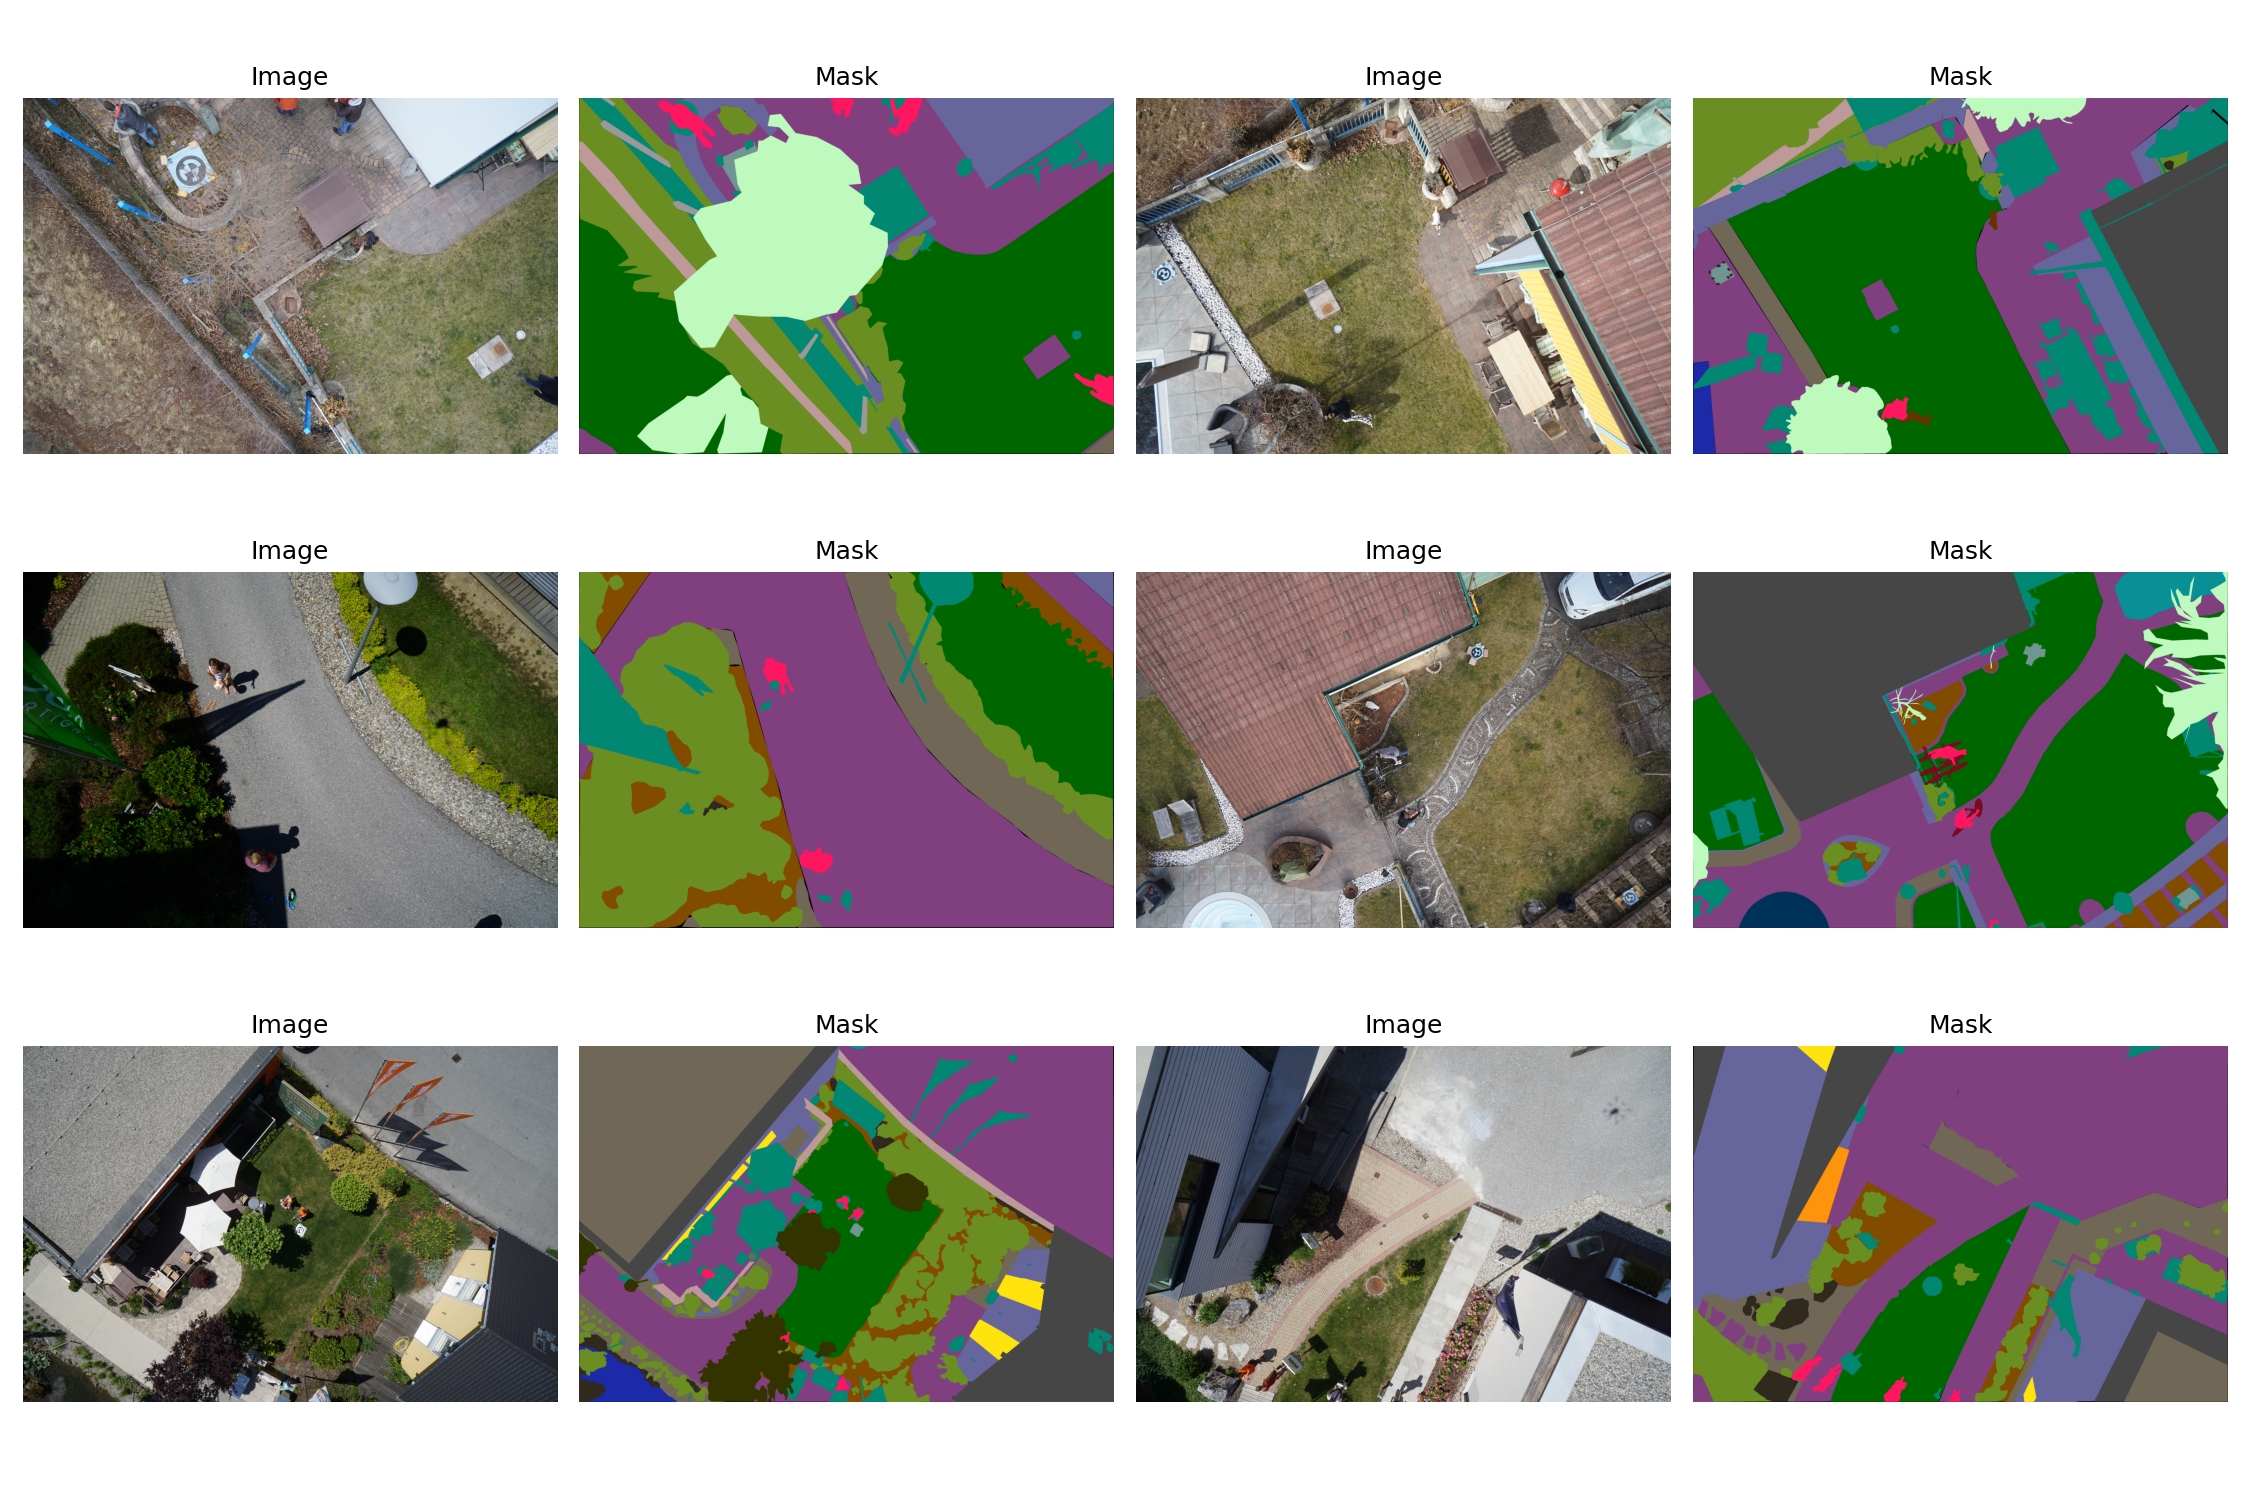
\includegraphics[width=\linewidth]{images/collection_1.png}
    \caption{Sample images and respective masks of the Semantic Drone Dataset.}
    \label{fig:collection_1}
\end{figure}

\subsection{Data Analysis and Preprocessing}
\subsection{Class Frequencies}
The dataset contains 23 classes, and their frequencies are shown in Table \ref{table:class_frequencies}. As expected for an urban area imagery dataset, there is significant class imbalance which is expected to impact the performance of the models, with less frequent classes presenting more challenges for accurate detection. The influence of this class imbalance on model performance will be analyzed in the \textit{Comparison of Per-Class IoU} section of the report.

\begin{table}[htbp]
    \centering
    \small
    \setlength{\tabcolsep}{5pt} % Adjust the value as needed
    \begin{tabular}{|l|r|r|}
    \hline
    \textbf{Class} & \textbf{Frequency} & \textbf{\%} \\ \hline
    paved-area     & $3.62 \times 10^9$ & 37.74 \\ \hline
    grass          & $1.92 \times 10^9$ & 19.98 \\ \hline
    roof           & $7.07 \times 10^8$ & 7.36 \\ \hline
    gravel         & $7.02 \times 10^8$ & 7.31 \\ \hline
    vegetation     & $6.82 \times 10^8$ & 7.10 \\ \hline
    obstacle       & $3.40 \times 10^8$ & 3.54 \\ \hline
    dirt           & $3.07 \times 10^8$ & 3.20 \\ \hline
    wall           & $2.58 \times 10^8$ & 2.69 \\ \hline
    water          & $2.12 \times 10^8$ & 2.21 \\ \hline
    tree           & $1.97 \times 10^8$ & 2.05 \\ \hline
    bald-tree      & $1.28 \times 10^8$ & 1.33 \\ \hline
    person         & $1.01 \times 10^8$ & 1.05 \\ \hline
    fence          & $9.20 \times 10^7$ & 0.96 \\ \hline
    car            & $7.55 \times 10^7$ & 0.79 \\ \hline
    rocks          & $6.90 \times 10^7$ & 0.72 \\ \hline
    pool           & $6.14 \times 10^7$ & 0.64 \\ \hline
    window         & $5.37 \times 10^7$ & 0.56 \\ \hline
    ar-marker      & $2.18 \times 10^7$ & 0.23 \\ \hline
    unlabeled      & $2.09 \times 10^7$ & 0.22 \\ \hline
    bicycle        & $2.07 \times 10^7$ & 0.22 \\ \hline
    fence-pole     & $5.10 \times 10^6$ & 0.05 \\ \hline
    door           & $3.01 \times 10^6$ & 0.03 \\ \hline
    dog            & $1.37 \times 10^6$ & 0.01 \\ \hline \hline
    \textbf{Total} & \textbf{$9.60 \times 10^9$} & \textbf{100}  \\ \hline 
    \end{tabular}
    \caption{Class frequencies and percentages.}
    \label{table:class_frequencies}
\end{table}

\subsubsection{Tiling}
The preprocessing of the dataset involved several steps to prepare the images for training. Initially, images were loaded and resized by rounding them down to the nearest multiple of the desired tile size. Various tile sizes were utilized, including 512, 768, 1000, and 2000 pixels. The number of tiles for each image and the total number of images for each tile size is shown in Table [\ref{table:number_of_tiles_and_total_tiles}]. After creating the tiles of different sizes, all tiles were further resized to 256x256 pixels to ensure consistency and computational efficiency during training. This tiling strategy allowed the model to process the images effectively by breaking them down into manageable segments, enhancing its ability to generalize across different regions of the images. The resized 256x256 pixels tiles were saved on disk, enabling faster data loading and processing during training, rather than performing tiling on-the-fly at each iteration.

\begin{table}[h]
\centering
\begin{tabular}{|c|c|c|}
\hline
\textbf{Tile Size (px)} & \textbf{Tiles/image} & \textbf{Total tiles} \\ \hline
512 x 512 & 77 & 30,800 \\ \hline
768 x 768 & 35 & 14,000 \\ \hline
1,000 x 1,000 & 24 & 9,600 \\ \hline
2,000 x 2,000 & 6 & 2,400 \\ \hline
\end{tabular}
\caption{Number of tiles per image and total tiles for tile size.}
\label{table:number_of_tiles_and_total_tiles}
\end{table}

\subsubsection{Image Augmentations}
Each image underwent a series of transformations during the \textit{\_\_getitem\_\_} function of the custom Dataset class. We leveraged the Albumentations library to perform these augmentations and by performing them during each iteration the dataset variability and training robustness was increased. The same set of transformations, with minor differences, was applied to both training and validation/test images to maintain consistency.

Augmentations included horizontal and vertical flips, brightness and contrast adjustments, and blur effects like Gaussian and motion blur. Color adjustments, including changes to hue, saturation, and value, were used to simulate different lighting conditions. CLAHE was applied to enhance contrast, and normalization ensured consistent pixel values across images.

The application of these augmentations improved the model's robustness by diversifying the training data, enhancing its ability to accurately segment diverse aerial images.

\section{Methodology}
\subsection{Network Architecture: DeepLabv3+}
In this study, we adopt the DeepLabv3+ architecture \cite{deeplabv3plus2018} for the task of semantic segmentation, due to its demonstrated ability to capture both global and local contextual information, which is crucial for generating precise segmentation maps. DeepLabv3+ enhances its predecessor, DeepLabv3 \cite{deeplab2016}, by introducing a decoder module that refines the resolution of the segmentation outputs, particularly at the boundaries of objects. This refinement is especially important in applications where accurately delineating the contours of objects, such as roads, buildings, and vegetation in urban drone imagery, is required.

A key innovation in DeepLabv3+ is the employment of atrous (or dilated) convolutions. \textit{Atrous convolutions} allow the model to maintain high spatial resolution while expanding the receptive field, enabling it to capture multi-scale contextual information without increasing the number of parameters. This approach is further enhanced by the \textit{Atrous Spatial Pyramid Pooling (ASPP)} module, which applies atrous convolutions at multiple rates, thereby improving the model's ability to recognize objects at varying scales and capture fine details across different regions of the image.

The \textit{encoder-decoder structure} of DeepLabv3+ plays a pivotal role in its performance. The encoder extracts deep features from the input image, which are then processed by the ASPP module before being fed into the decoder. The decoder subsequently refines the segmentation map, leading to sharper and more accurate predictions.

\subsection{Encoders}
For the DeepLabv3+ backbone of our network architecture, three different encoders were selected: EfficientNetB5, ResNet34, and MobileNetV2. Each encoder was chosen to balance various aspects of performance and computational efficiency to suit different operational needs. A brief overview of the number of trainable parameters for these encoders is provided in Table [\ref{table:encoders}].

\begin{table}[h]
\centering
\begin{tabular}{|c|c|c|}
\hline
\textbf{Encoder} & \textbf{\# Parameters} \\ \hline
MobileNetV2 & 3.4M \\ \hline
ResNet34 & 21.8M \\ \hline
EfficientNet-B5 & 28.3M \\ \hline
\end{tabular}
\caption{Number of trainable parameters}
\label{table:encoders}
\end{table}

\subsubsection{EfficientNetB5}
EfficientNetB5 is a highly efficient convolutional neural network that uses compound scaling to balance depth, width, and resolution, optimizing both accuracy and computational efficiency \cite{efficientnet2019}. Its architecture incorporates mobile inverted bottleneck convolution (MBConv) layers, enhancing feature extraction while keeping the model lightweight.

\subsubsection{ResNet34}
ResNet34 is a deeper residual network that offers a strong balance between depth and computational efficiency. Its architecture incorporates residual connections to overcome the vanishing gradient problem, allowing for effective training of deeper models \cite{resnet2016}. ResNet34's increased depth enables it to capture complex features and intricate details, making it well-suited for comprehensive segmentation tasks, including those involving detailed urban imagery.

\subsubsection{MobileNetV2}
MobileNetV2 is designed specifically for environments where computational resources are constrained, such as mobile and edge devices \cite{mobilenetv22018}. It employs depthwise separable convolutions and an inverted residual structure with linear bottlenecks to reduce model size and computational demands while maintaining high accuracy. MobileNetV2 is particularly advantageous for real-time applications on drones, where efficiency and rapid processing are critical.

\subsection{Training}
During the training process, we utilize the \textit{CrossEntropyLoss} as the loss function, which is well-suited for multi-class segmentation tasks. The \textit{AdamW} optimizer is selected due to its enhanced generalization capabilities and better performance in preventing overfitting compared to the standard Adam optimizer. The learning rate is adjusted using a \textit{Cosine Annealing} strategy, with the learning rate being periodically reset every 25 epochs. This approach helps in escaping local minima and facilitates a more thorough exploration of the loss landscape. For each encoder and tiles dimension configuration, the training procedure involves monitoring the model's performance on a validation set at the end of each epoch. The model with the lowest validation loss is saved as a best model checkpoint for that configuration. Finally, the best models are evaluated on the test set. 

\subsection{Evaluation Metrics}
For the evaluation of the trained models, several metrics are computed to comprehensively assess their performance. These metrics include:
\begin{itemize}
    \item \textbf{Weighted Mean Dice:} This metric is calculated based on the class frequencies in the validation set to account for class imbalance. The Dice coefficient measures the overlap between the predicted and ground truth segmentation masks.

    \item \textbf{Weighted Mean Intersection over Union (IoU):} Similar to the weighted mean Dice, the weighted mean IoU is calculated with weights corresponding to the class frequencies in the validation set. The IoU measures the ratio of the intersection between the predicted and ground truth segmentation masks to their union, offering a more stringent evaluation of the model's performance.

    \item \textbf{Accuracy:} Overall accuracy is computed as the ratio of correctly classified pixels to the total number of pixels.

    \item \textbf{Per-Class IoU:} A per-class IoU is computed to analyze the model's strengths and weaknesses on the different classes.
\end{itemize}

\section{Results}
\subsection{Comparison of Accuracy, mean IoU and mean Dice}
The performance analysis across different encoders and tile dimensions, shown in Table \ref{table:performance_metrics}, reveals that \textbf{all the models performed the best with tiles of 512x512 pixels.}

Among the models, \textit{EfficientNet-B5} delivered the highest scores across all metrics. At 512x512 pixels, EfficientNet-B5 recorded an accuracy of 93.32\%, an mIoU of 88.87\%, and a mean Dice coefficient of 93.24\%. These results indicate that EfficientNet-B5 is highly effective at capturing detailed features, making it particularly suitable for tasks requiring high precision.

However, it is important to note that \textbf{MobileNetV2's performance was remarkably close to that of EfficientNet-B5}, despite its lighter architecture of 3.4 millions trainable parameters against EfficientNet-B5's 28.3 millions. At the same tile size of 512x512 pixels, MobileNetV2 achieved an accuracy of 92.89\%, an mIoU of 88.04\%, and a mean Dice coefficient of 92.65\%. These scores are only about 1\% lower than those of EfficientNet-B5, highlighting MobileNetV2's efficiency and possible use on devices with limited computing power such as drones.

ResNet34 also performed well, particularly at the 512x512 pixel tile size, with an accuracy of 93.27\%, an mIoU of 88.64\%, and a mean Dice coefficient of 93.05\%. While ResNet34's performance was strong, it did not significantly surpass that of MobileNetV2, further emphasizing how well MobileNetV2 balances performance and efficiency.

\begin{table}[htbp]
    \centering
    \small
    \begin{tabular}{|l|r|r|r|r|}
    \hline
    \textbf{Encoder} & \textbf{Tiles} & \textbf{Accuracy} & \textbf{mIoU} & \textbf{mDice} \\ \hline
     ResNet34 & \textbf{512} & \textbf{93.27} & \textbf{88.64} & \textbf{93.05} \\ \hline
    ResNet34 & 768 & 93.17 & 88.36 & 92.94 \\ \hline
    ResNet34 & 1000 & 90.97 & 84.89 & 90.73 \\ \hline
    ResNet34 & 2000 & 88.90 & 81.36 & 88.56 \\ \hline
    EfficientNet-B5 & \textbf{512} & \textbf{93.32} & \textbf{88.87} & \textbf{93.24} \\ \hline
    EfficientNet-B5 & 768 & 92.63 & 87.64 & 92.50 \\ \hline
    EfficientNet-B5 & 1000 & 91.53 & 85.70 & 91.27 \\ \hline
    EfficientNet-B5 & 2000 & 90.79 & 84.35 & 90.58 \\ \hline
    MobileNetV2 & \textbf{512} & \textbf{92.89} & \textbf{88.04} & \textbf{92.65} \\ \hline
    MobileNetV2 & 768 & 91.90 & 86.32 & 91.61 \\ \hline
    MobileNetV2 & 1000 & 90.89 & 84.65 & 90.58 \\ \hline
    MobileNetV2 & 2000 & 89.14 & 81.74 & 88.79 \\ \hline
    \end{tabular}
    \caption{Final performance metrics for different encoders and tiles dimensions in pixel. Accuracy, weighted mean IoU (mIoU) and weighted mean Dice (mDice) are expressed as percentages \%.}
    \label{table:performance_metrics}
\end{table}

\subsection{Comparison of Per-class IoU}
The per-class Intersection over Union (IoU) analysis provides a detailed comparison of the three best-performing network configurations on 512x512 pixel tiles. The results, presented in Table [\ref{table:per_class_iou}], highlight the strengths and limitations of each model across various semantic categories.. 

EfficientNet-B5 consistently outperformed the other models in most classes, achieving the highest IoU in 13 out of the 23 classes. ResNet34 also performed well, particularly in classes such as 'dirt' and 'pool,' where it marginally surpassed EfficientNet-B5.

\textit{MobileNetV2 delivered remarkably close results to the other two models}, despite being the smallest model with only 3.4 million parameters. In many classes, the IoU difference between MobileNetV2 and the best-performing model was minimal, often within 1\%. This \textit{balance} between model size and performance underscores MobileNetV2’s potential for deployment in resource-constrained environments, such as drones, where both computational efficiency and high segmentation accuracy are essential.

\begin{table}[htbp]
    \centering
    \small
    \setlength{\tabcolsep}{5pt} % Adjust the value as needed
    \begin{tabular}{|l|r|r|r|}
    \hline
    \textbf{Class} & \textbf{EffNet-B5} & \textbf{ResNet34} & \textbf{MobNetV2} \\ \hline
    paved-area     & \textbf{95.25\%} & 95.13\% & 94.53\% \\ \hline
    grass          & 93.89\% & 94.10\% & \textbf{94.66\%} \\ \hline
    roof           & 82.88\% & \textbf{83.82\%} & 77.18\% \\ \hline
    gravel         & 80.14\% & \textbf{82.19\%} & 81.39\% \\ \hline
    vegetation     & \textbf{70.00\%} & 68.57\% & 66.36\% \\ \hline
    obstacle       & 64.72\% & \textbf{64.76\%} & 60.49\% \\ \hline
    dirt           & 53.32\% & \textbf{55.03\%} & 53.61\% \\ \hline
    wall           & \textbf{62.27\%} & 57.67\% & 56.80\% \\ \hline
    water          & 50.58\% & 48.66\% & \textbf{51.94\%} \\ \hline
    tree           & \textbf{46.20\%} & 45.46\% & 40.69\% \\ \hline
    bald-tree      & 28.88\% & \textbf{31.88\%} & 28.88\% \\ \hline
    person         & \textbf{64.78\%} & 62.29\% & 56.56\% \\ \hline
    fence          & \textbf{37.49\%} & 35.98\% & 33.22\% \\ \hline
    car            & \textbf{29.90\%} & 26.39\% & 29.53\% \\ \hline
    rocks          & \textbf{34.42\%} & 31.64\% & 31.92\% \\ \hline
    pool           & 27.99\% & \textbf{28.95\%} & 24.49\% \\ \hline
    window         & 26.09\% & \textbf{26.87}\% & 22.78\% \\ \hline
    ar-marker      & \textbf{24.80\%} & 20.93\% & 21.04\% \\ \hline
    unlabeled      & 0.35\%  & \textbf{0.54\%}  & 0.29\%  \\ \hline
    bicycle        & \textbf{18.98\%} & 16.86\% & 17.48\% \\ \hline
    fence-pole     & \textbf{5.01\%}  & 4.81\%  & 4.06\%  \\ \hline
    door           & \textbf{1.01\%}  & 0.55\%  & 0.46\%  \\ \hline
    dog            & 3.47\%  & 3.10\%  & \textbf{3.48\%}  \\ \hline
    \end{tabular}
    \caption{Per class IoU comparison for EfficientNet-B5, ResNet34, and MobileNetV2. Values are expressed as percentages.}
    \label{table:per_class_iou}
\end{table}

\subsection{Qualitative Results}

Figures [\ref{fig:grid_287_@512px_efficientnet-b5_with_legend}], [\ref{fig:grid_287_@512px_resnet34_with_legend}], and [\ref{fig:grid_287_@512px_mobilenet_v2_with_legend}] present a qualitative comparison of the segmentation performance of EfficientNet-B5, ResNet34, and MobileNetV2, respectively, using 512x512 pixel tiles. Each figure displays a 2x3 grid layout, comprising the original image, ground truth mask, predicted mask, model confidence map, overlaid mask on the original image, and a difference mask that highlights the regions of incorrect predictions.

\textit{Both EfficientNet-B5 and MobileNetV2 demonstrate a high degree of accuracy in their predicted masks}. The difference masks reveal that most misclassifications happen along the object boundaries, which are typically challenging areas for segmentation models. Notably, MobileNetV2, despite its smaller size, delivers competitive performance that is comparable to its more complex counterparts, underscoring its efficiency and potential applicability in resource-constrained environments such as deployment on drones.

\begin{figure*}[!htbp]
    \centering
    \begin{minipage}{\textwidth}
        \centering
        \includegraphics[width=0.8\textwidth]{images/grid_544_512px_efficientnet-b5_with_legend.png}
        \caption{EfficientNet-B5 @ 512 pixels: Original Image, Ground Truth Mask, Predicted Mask, Model Confidence, Overlaid Mask, and Difference Mask.}
        \label{fig:grid_544_@512px_efficientnet-b5_with_legend}
    \end{minipage}
    
    \vspace{0pt} % Add some space between figures if needed
    
    \begin{minipage}{\textwidth}
        \centering
        \includegraphics[width=0.8\textwidth]{images/grid_544_512px_resnet34_with_legend.png}
        \caption{ResNet34 @ 512 pixels: Original Image, Ground Truth Mask, Predicted Mask, Model Confidence, Overlaid Mask, and Difference Mask.}
        \label{fig:grid_544_@512px_resnet34_with_legend}
    \end{minipage}
    
    \vspace{0pt} % Add some space between figures if needed
    
    \begin{minipage}{\textwidth}
        \centering
        \includegraphics[width=0.8\textwidth]{images/grid_544_512px_mobilenet_v2_with_legend.png}
        \caption{MobileNetV2 @ 512 pixels: Original Image, Ground Truth Mask, Predicted Mask, Model Confidence, Overlaid Mask, and Difference Mask.}
        \label{fig:grid_544_@512px_mobilenet_v2_with_legend}
    \end{minipage}
\end{figure*}

% \begin{figure*}[!htbp]
%     \centering
%     \begin{minipage}{\textwidth}
%         \centering
%         \includegraphics[width=0.8\textwidth]{images/grid_544_768px_efficientnet-b5_with_legend.png}
%         \caption{EfficientNet-B5 @ 768 pixels: Original Image, Ground Truth Mask, Predicted Mask, Model Confidence, Overlaid Mask, and Difference Mask.}
%         \label{fig:grid_544_@768px_efficientnet-b5_with_legend}
%     \end{minipage}
    
%     \vspace{0pt} % Add some space between figures if needed
    
%     \begin{minipage}{\textwidth}
%         \centering
%         \includegraphics[width=0.8\textwidth]{images/grid_544_768px_resnet34_with_legend.png}
%         \caption{ResNet34 @ 768 pixels: Original Image, Ground Truth Mask, Predicted Mask, Model Confidence, Overlaid Mask, and Difference Mask.}
%         \label{fig:grid_544_@768px_resnet34_with_legend}
%     \end{minipage}
    
%     \vspace{0pt} % Add some space between figures if needed
    
%     \begin{minipage}{\textwidth}
%         \centering
%         \includegraphics[width=0.8\textwidth]{images/grid_544_768px_mobilenet_v2_with_legend.png}
%         \caption{MobileNetV2 @ 768 pixels: Original Image, Ground Truth Mask, Predicted Mask, Model Confidence, Overlaid Mask, and Difference Mask.}
%         \label{fig:grid_544_@768px_mobilenet_v2_with_legend}
%     \end{minipage}
% \end{figure*}

\section{Discussion on Drone Deployment}

Deploying deep learning models for real-time semantic segmentation on drones presents significant challenges, primarily due to the limited computational resources available on-board. Although MobileNetV2 is designed for efficiency on edge devices, its performance may still be constrained by the restricted processing power and battery capacity of drones.

During testing, MobileNetV2 achieved approximately 41 frames per second (fps) on a Nvidia RTX 3060 Ti GPU. However, this performance would likely decrease significantly when deployed on a drone, which could limit its effectiveness in real-time segmentation tasks. \textit{Several strategies can be considered to mitigate these limitations.}

\subsection{Remote Image Processing}

One approach is to offload the image processing tasks to a nearby ground station or cloud server. By transmitting raw image data to a more powerful computing system, the drone’s computational burden can be reduced. This approach takes advantage of external resources to perform segmentation and then sends the processed results back to the drone. While effective, this method relies on a stable communication link and may introduce latency.

\subsection{Frame Rate Reduction}

Another viable strategy is to decrease the frame rate of the drone’s camera. Since the objects of interest in an urban area are typically static or change slowly, processing fewer frames per second can significantly lower the computational demand. This trade-off can help conserve battery life and maintain operational efficiency while still achieving accurate segmentation results.

\subsection{Model Quantization}

Model quantization is an effective technique to address the computational challenges of deploying neural networks on drones. This process involves converting a model’s floating-point weights and activations into lower precision formats, such as integers, which reduces both the model’s size and its computational requirements \cite{han2016}. Quantization enhances the model’s efficiency, making it more suitable for real-time applications on resource-constrained devices like drones. In addition to quantization, model pruning is a valuable technique. This method reduces the number of connections within the network by keeping only the most essential ones, thus simplifying the model.

\textit{The deep compression technique \cite{han2016}, which combines pruning, quantization, and Huffman coding, can substantially reduce the storage and computational needs of neural networks.} Pruning alone can decrease the number of connections by 9× to 13×, and quantization can further compress the model by reducing the bit-width of weights from 32 bits to as few as 5 bits, significantly decreasing model size.

For example, the deep compression technique has demonstrated a reduction in model storage by 35× for AlexNet, from 240MB to 6.9MB, and by 49× for VGG-16, from 552MB to 11.3MB, without sacrificing accuracy. This compression allows models to fit within on-chip SRAM caches rather than relying on off-chip DRAM memory. Additionally, compressed models exhibit 3× to 4× layer-wise speedup and 3× to 7× improvements in energy efficiency, which translates to enhanced battery life and computational performance on various hardware platforms, including mobile GPUs \cite{han2016}.

Incorporating these compression techniques can make models like MobileNetV2 more viable for drone deployment, optimizing both computational efficiency and practical application.

\section{Discussion on Tile Size}
\textbf{Small Tile Size Wins: }All models performed best with tiles of 512x512 pixels, indicating that smaller tile sizes are more effective for capturing detailed features and improving segmentation accuracy. Many classes in the dataset consist of small objects at the drone altitude (e.g., person, window, door, dog). Given that all tiles are resized to 256x256 pixels, the 512x512 pixel tiles capture the most detailed features. However, a larger tile size (for example, 768x768 pixels) could provide a better balance in terms of computational requirements and accuracy, as it reduces the number of tiles per image by half, resulting in only about a 1\% decrease in performance (35 tiles at 768x768 pixels versus 77 tiles at 512x512 pixels). Increasing the tile size further to 1,000x1,000 pixels could lower the computational requirements of the network by a factor of 3, decreasing the number of tiles from 77 per image to 24. This reduction would lead to higher frames per second (FPS) for detection. The choice of optimal tile dimensions ultimately depends on the application's priorities: whether to prioritize higher accuracy at the expense of FPS or to accept slightly lower accuracy for improved FPS.

\section{Conclusion}
This study conducted a comprehensive evaluation of the DeepLabv3+ architecture using EfficientNet-B5, ResNet34, and MobileNetV2 encoders for semantic segmentation of urban drone imagery, focusing on the Semantic Drone Dataset. Our findings reveal several key insights:

\begin{itemize}
    \item \textbf{Small Tile Size Wins:} All models performed best with tiles of 512x512 pixels. However, these tile dimensions impose significant computational requirements due to the high number of tiles per image (77 tiles). Larger tile sizes, such as 768x768 pixels or 1,000x1,000 pixels, offer nearly equivalent performance while reducing the number of tiles per image by a factor of 2 or 3, respectively, thereby maintaining high performance with lower computational demands.
    \item \textbf{EfficientNet-B5} consistently delivered the highest scores across all metrics, achieving an accuracy of 93.32\%, an mIoU of 88.87\%, and a mean Dice coefficient of 93.24\% at 512x512 pixels. \textbf{ResNet34} followed closely, with an accuracy of 93.27\%, an mIoU of 88.64\%, and a mean Dice coefficient of 93.05\%. However, these larger models are not fit for running on drones due to the limited computing power and battery on-board.
    \item \textbf{MobileNetV2} demonstrated a remarkable balance between performance and efficiency, achieving an accuracy of 92.89\%, an mIoU of 88.04\%, and a mean Dice coefficient of 92.65\% at 512x512 pixels. The differences in performance metrics between EfficientNet-B5 and MobileNetV2 are shown in Table [\ref{tab:delta_table}], with the delta consistently smaller than 1\%. Despite its lighter architecture, MobileNetV2's performance was impressively close to that of EfficientNet-B5, making it particularly well-suited for applications in drone autonomous driving that require rapid, on-the-fly image analysis.
\end{itemize}

\begin{table}[!htbp]
    \centering
    \begin{tabular}{|c|r|r|r|}
    \hline
     Metric    &  EffNet-B5 & MobNetV2 & Delta \\ \hline
     Accuracy    &  93.32 & 92.89 & 0.43 \\ \hline
     Mean IoU    &  88.87 & 88.04 & 0.83 \\ \hline
     Mean Dice    & 93.24 & 92.65 & 0.59 \\ \hline
    \end{tabular}
    \caption{Performance comparison across different metrics (expressed as percentages \%) of EfficientNet-B5 and MobileNetV2 with tiles of 512x512 pixels. Notice that the delta is smaller than 1\%.}
    \label{tab:delta_table}
\end{table}

However, deploying MobileNetV2 on drones presents challenges due to the limited on-board resources. To address this, the following possible solutions require further studies and testing:

\begin{itemize}
    \item Implementing remote image processing to offload computational tasks to ground stations or cloud servers.
    \item Reducing frame rates to decrease computational load while maintaining effective segmentation for slowly changing scenes.
    \item Applying model quantization and pruning techniques to further optimize model size and computational efficiency without significant loss in accuracy.
\end{itemize}

These strategies can help bridge the gap between the high accuracy of larger models like EfficientNet-B5 or ResNet34 and the computational requirements of drone-based applications.

In conclusion, while EfficientNet-B5 offers marginally superior segmentation accuracy, MobileNetV2 emerges as a highly promising solution for drone-based urban imagery analysis. Its balance of efficiency and performance, coupled with appropriate deployment strategies, positions it well for real-world applications of autonomous navigation of drones in urban areas, such as for drone deliveries, and for infrastructure inspection. Future research should focus on further optimizing these models for edge devices and exploring hybrid approaches that combine the strengths of different architectures for specific deployment scenarios.

\bibliographystyle{ieeetr} % or any other style you prefer, like plain, alpha, etc.
\bibliography{references}

\end{document}
